\documentclass[12pt]{article}

\usepackage{amsmath, mathtools}
\usepackage{amsfonts}
\usepackage{amssymb}
\usepackage{graphicx}
\usepackage{colortbl}
\usepackage{xr}
\usepackage{hyperref}
\usepackage{longtable}
\usepackage{xfrac}
\usepackage{tabularx}
\usepackage{float}
\usepackage{siunitx}
\usepackage{booktabs}
\usepackage{caption}
\usepackage{pdflscape}
\usepackage{afterpage}
\usepackage{tabu}
\usepackage{verbatim}
\usepackage[round]{natbib}
\usepackage{url}
\usepackage{tikz}
\usetikzlibrary{shapes.geometric, arrows}

\captionsetup{belowskip=12pt,aboveskip=4pt}

\makeatletter
\newcommand*\bigcdot{\mathpalette\bigcdot@{.7}}
\newcommand*\bigcdot@[2]
  {\mathbin{\vcenter{\hbox{\scalebox{#2}{$\m@th#1\bullet$}}}}}
\makeatother

%\usepackage{refcheck}

\hypersetup{
    bookmarks=true,         % show bookmarks bar?
      colorlinks=true,      % false: boxed links; true: colored links
    linkcolor=red,          % color of internal links 
                            %  (change box color with linkbordercolor)
    citecolor=blue,        % color of links to bibliography
    filecolor=magenta,      % color of file links
    urlcolor=cyan           % color of external links
}

%% Comments

\usepackage{color}

\newif\ifcomments\commentsfalse

\ifcomments
\newcommand{\authornote}[3]{\textcolor{#1}{[#3 ---#2]}}
\newcommand{\todo}[1]{\textcolor{red}{[TODO: #1]}}
\else
\newcommand{\authornote}[3]{}
\newcommand{\todo}[1]{}
\fi

\newcommand{\wss}[1]{\authornote{blue}{SS}{#1}}
\newcommand{\spc}[1]{\authornote{magenta}{SP}{#1}}


\newcommand{\sskip}{\vskip 1mm}

% For easy change of table widths
\newcommand{\colZwidth}{1.0\textwidth}
\newcommand{\colAwidth}{0.13\textwidth}
\newcommand{\colBwidth}{0.82\textwidth}
\newcommand{\colCwidth}{0.1\textwidth}
\newcommand{\colDwidth}{0.05\textwidth}
\newcommand{\colEwidth}{0.8\textwidth}
\newcommand{\colFwidth}{0.17\textwidth}
\newcommand{\colGwidth}{0.5\textwidth}
\newcommand{\colHwidth}{0.28\textwidth}

% Used so that cross-references have a meaningful prefix
\newcounter{defnum} %Definition Number
\newcommand{\dthedefnum}{GD\thedefnum}
\newcommand{\dref}[1]{GD\ref{#1}}
\newcounter{datadefnum} %Datadefinition Number
\newcommand{\ddthedatadefnum}{DD\thedatadefnum}
\newcommand{\ddref}[1]{DD\ref{#1}}
\newcounter{theorynum} %Theory Number
\newcommand{\tthetheorynum}{T\thetheorynum}
\newcommand{\tref}[1]{T\ref{#1}}
\newcounter{tablenum} %Table Number
\newcommand{\tbthetablenum}{T\thetablenum}
\newcommand{\tbref}[1]{TB\ref{#1}}
\newcounter{assumpnum} %Assumption Number
\newcommand{\atheassumpnum}{P\theassumpnum}
\newcommand{\aref}[1]{A\ref{#1}}
\newcounter{goalnum} %Goal Number
\newcommand{\gthegoalnum}{P\thegoalnum}
\newcommand{\gsref}[1]{GS\ref{#1}}
\newcounter{instnum} %Instance Number
\newcommand{\itheinstnum}{IM\theinstnum}
\newcommand{\iref}[1]{IM\ref{#1}}
\newcounter{reqnum} %Requirement Number
\newcommand{\rthereqnum}{P\thereqnum}
\newcommand{\rref}[1]{R\ref{#1}}
\newcounter{nfreqnum} %NF Requirement Number
\newcommand{\rthenfreqnum}{P\thenfreqnum}
\newcommand{\nfref}[1]{NF\ref{#1}}
\newcounter{lcnum} %Likely change number
\newcommand{\lthelcnum}{LC\thelcnum}
\newcommand{\lcref}[1]{LC\ref{#1}}
\newcommand{\sref}[1]{\S~\ref{#1}}

\usepackage{fullpage}

\begin{document}
\pagenumbering{gobble}

\title{CAS 741: SRS\\[10pt]\Large Dynamical Systems: Multi-Pendulum}
\author{Karol Serkis\\\texttt{serkiskj@mcmaster.ca}}
\date{\today}
	
\maketitle

~\newpage

\pagenumbering{roman}
\tableofcontents

\clearpage

\setcounter{secnumdepth}{0}

\section{Revision History}

\begin{table}[hp]
\caption{Revision History}
\begin{tabularx}{\textwidth}{llX}
\toprule
\textbf{Date} & \textbf{Developer(s)} & \textbf{Change}\\
\midrule
September 28, 2018 & Karol Serkis & First revision of document in landscape orientation for presentation\\
September 26, 2018 & Karol Serkis & SRS presentation slides discussed with Dr. Spencer Smith \\
\bottomrule
\end{tabularx}
\end{table}

~\newpage

\section{Reference Material}

\subsection{Mathematical Notation}

This section describes the notation conventions used in this document.

\begin{figure}[H]
	\centering
	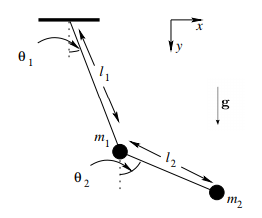
\includegraphics[width=200px]{doublepend.PNG}
	\caption{A simple gravity double pendulum (model assumes no friction or air resistance)}
	\label{fig:maxresdefault}
\end{figure}

$$x_1 = l_1 \sin\theta_1 \quad\quad y_1 = -l_1 \cos\theta_1$$
$$x_2 = l_1 \sin\theta_1 + l_2 \sin\theta_2 \quad\quad y_2 = -l_1\cos\theta_1 -l_2\cos\theta_2$$


\subsection{Table of Units}

Throughout this document SI (Syst\`{e}me International d'Unit\'{e}s) is employed 
as the unit system.  In addition to the basic units, several derived units are
used as described below.  For each unit, the symbol is given followed by a
description of the unit and the SI name.\\

\renewcommand{\arraystretch}{1.2}
  \noindent \begin{tabular}{l l l} 
    \toprule		
    \textbf{symbol} & \textbf{unit} & \textbf{SI}\\
    \midrule 
    \si{\metre} & length & metre\\
    \si{\kilogram} & mass & kilogram\\
    \si{\second} & time & second\\
    \bottomrule
  \end{tabular}

\newpage

\subsection{Table of Symbols}

The table that follows summarizes the symbols used in this document along with
their units.  The choice of symbols was made to be consistent with calculus, ordinary differentials (ODE), Lagrangian, kinematics etc.  The symbols are listed in alphabetical order.
~\newline
\renewcommand{\arraystretch}{1.2}
%\noindent \begin{tabularx}{1.0\textwidth}{l l X}
\noindent \begin{longtable*}{l l l p{8cm}} \toprule
\textbf{symbol} & \textbf{space} & \textbf{unit} & \textbf{description}\\
\midrule 
$\theta$ & $\mathbb{N}$ & -- & amplitude from the pivot point
\\
$g$ & $\mathbb{N}$ & -- & gravitational constant
\\
$m_1$ & $\mathbb{N}$ & -- & mass of the 1st pendulum weight
\\ 
$m_2$ & $\mathbb{N}$ & -- & mass of the 2nd pendulum weight
\\ 
$m_n$ & $\mathbb{N}$ & -- & mass of the nth pendulum weight
\\ 
$x_1$ & $\mathbb{N}$ & -- & length of the 1st pendulum rod
\\ 
$x_2$ & $\mathbb{N}$ & -- & length of the 2nd pendulum rod
\\ 
$x_n$ & $\mathbb{N}$ & -- & length of the nth pendulum rod
\\
\bottomrule
\end{longtable*}


\subsection{Abbreviations and Acronyms}

\renewcommand{\arraystretch}{1.2}
\begin{tabular}{l l} 
  \toprule		
  \textbf{symbol} & \textbf{description}\\
  \midrule 
  A & Assumption\\
  DD & Data Definition\\
  GD & General Definition\\
  GS & Goal Statement\\
  IM & Instance Model\\
  LC & Likely Change\\
  NF & Non-Functional Requirement\\
  PS & Physical System Description\\
  R & Requirement\\
  SRS & Software Requirements Specification\\
  T & Theoretical Model\\
  \bottomrule
\end{tabular}\\

\newpage

\pagenumbering{arabic}

\setcounter{secnumdepth}{3}

\section{Introduction}

\subsection{Purpose of Document}
The purpose of this document is to describe the requirements for a
Multi-Pendulum Simulation program, a  multi-platform equivalent solution that
only focuses on multi-pendulum simulations and tracking the chaotic motion of
the system. It will allow users to generate diagrams and plot trajectories over
time using two different ODE/DAE initial value problem solvers. In the case of 
a double pendulum you have a new system that is dynamic and chaotic and requires
a set of coupled ordinary differential equation solvers. Once you introduce multiple
pendula the system becomes chaotic and interesting to model and simulate. 
The simulation software will be created with multi-platform support.

The goals and models used in the Multi-Pendulum code will be provided, insuring
assumptions and unambiguous definitions are itentified. This document 
is intended to be used as a reference to provide all information necessary to 
understand and verify the inputs to outputs. The SRS is abstract: the contents 
describe the problem being solved, but not how to solve it.

This document will be used as a starting point for subsequent development
phases, including writing the design specification and the software verification
and validation plan. The verification and validation plan will show the steps in 
the software documentation/implementation.

\wss{The text is better for version control, and for reading in other editors,
  if you use a hard-wrap at 80 characters}

\subsection{Scope of Requirements} 

The scope of the Multi-Pendulum Simulation program is limited to the generation 
of diagrams and plot trajectories that are possible to run and compute on a local system.\\

Assumptions: No server-side processing or parallel/distributed computing will be utilized.
The multi-pendulum simulation will be a closed system. Air resistance and friction will 
not be considered for the simulation.\\

Question: Should the implementation be limited to local systems? Should a mobile-ready 
implementation be made for lower performance systems? What do I mean by multi-platform implementation?

\subsection{Characteristics of Intended Reader} 
The intended reader is expected to have a minimum knowledge in mathematics and physics at
undergraduate level. Simplification of some physical concepts are proposed to
make the document technically accessible. Nevertheless, a basic knowledge in
mathematics (calculus, differentials) and physics (kinematics, energy potential, Lagrangian) is 
recommended to get a deeper understanding of the document.

\subsection{Organization of Document}
\begin{itemize}
\item The organization of this document follows the template for an SRS for scientific 
computing software proposed by Dr. Spencer Smith. 
\item The presentation follows the standard pattern of presenting goals, theories, definitions, and assumptions. 
\item The goal statements are refined to the theoretical models, and the theoretical 
models to the instance models. The data definitions are used to support the definitions of the different models.
\end{itemize}
\newpage
\section{General System Description}
This section identifies the interfaces between the system and its environment,
describes the user characteristics and lists the system constraints.

\subsection{System Context}

\tikzstyle{startstop} = [rectangle, rounded corners, minimum width=3cm, minimum height=1cm,text centered, draw=black, fill=red!30]
\tikzstyle{process} = [rectangle, minimum width=3cm, minimum height=2cm, text centered, draw=black, fill=orange!30]
\tikzstyle{decision} = [diamond, minimum width=3cm, minimum height=2cm, text centered, draw=black, fill=green!30]

\begin{tikzpicture}[node distance=2cm]
\node (start) [startstop] {User}; 
\end{tikzpicture}
\begin{tikzpicture}[node distance=2cm]
\draw (0,0) -- (1,1);
\end{tikzpicture}
\begin{tikzpicture}[node distance=2cm]
\node (pro1) [process, below of=start] {Multi-Pendulum};
\end{tikzpicture}
\begin{tikzpicture}[node distance=2cm]
\draw (0,0) -- (1,1);
\end{tikzpicture}
\begin{tikzpicture}[node distance=2cm]
\node (end) [startstop, below of=pro1] {User};
\end{tikzpicture}

\begin{itemize}
\item User Responsibilities:
\begin{itemize}
\item Ensure that the input data is fits the system model.
\item Ensure that the input data is within scope.
\end{itemize}
\item Multi-Pendulum Simulation program Responsibilities:
\begin{itemize}
\item Detect data type mismatch, such as a string of characters instead of a
  floating point number.
\item Determine if the inputs satisfy the required physical and software 
  constraints.
\item Solve the system of equations arising from the input data to generate 
  the output data.
\item Generate a plot of the output data.
\end{itemize}
\end{itemize}

\subsection{User Characteristics}
The end user of Multi-Pendulum Simulation program should have an understanding of first year 
undergraduate math and physics. Less understanding of physics and math are required to use the software.

\subsection{System Constraints}
There are no system constraints.

\newpage
\section{Specific System Description}

This section first presents the problem description, which gives a high-level
view of the problem to be solved.  This is followed by the solution 
characteristics specification, which presents the assumptions, theories, 
definitions and finally the instance models.

\subsection{Problem Description}
A simple gravity pendulum has very easy to system to model and consists of a
weight suspended from a pivot and the weight is given enough space to swing
freely. To simplify the model we assume no air resistance with a frictionless
pivot. The model and calculations for the simple gravity pendulum are well
defined and only require simple derivations and differential solvers.

Multi-Pendulum Simulation program will produce a simulation given a set of equilibrium constants and input. 

\subsubsection{Terminology and Definitions}

This subsection provides a list of terms that are used in the subsequent
sections and their meaning, with the purpose of reducing ambiguity and making it
easier to correctly understand the requirements:

\begin{description}
\item[Lagrangian:] the $L=T-V$, where T and V are the kinetic and potential energies of the system respectively.
\item[Equilibrium position:] the pendulum rod and weight position in its resting state.
\item[3D Cartesian coordinate system:] the pendulum rod and weight swing from a pivot position origin $(x,y,z)$
\end{description}

\begin{figure}[H]
	\centering
	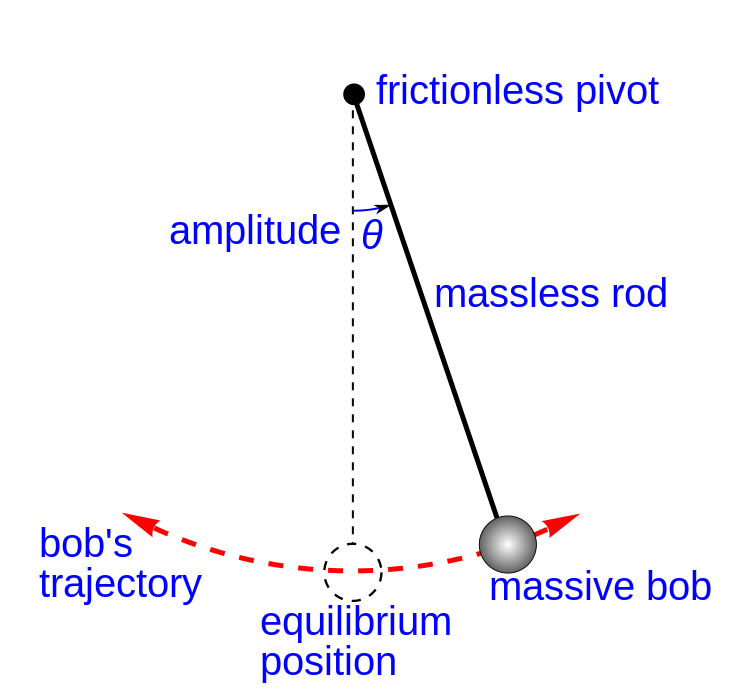
\includegraphics[width=190px]{simple-pend.png}
	\caption{A simple gravity pendulum where the model assumes no friction or air resistance}
	\label{fig:maxresdefault}
\end{figure}

\subsubsection{Physical System Description}

The physical system of Multi-Pendulum Simulation program includes the following elements:

\begin{itemize}
\item[PS1:] Simulate an n-rod Multi-Pendulum system with no friction and no air resistance in a 3D space.
\end{itemize}

\begin{figure}[H]
	\centering
	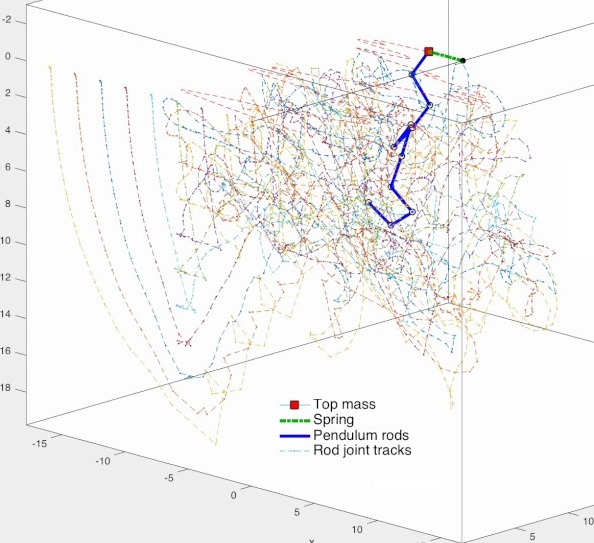
\includegraphics[width=430px]{multi-pend.jpg}
	\caption{An example of dynamical and chaoitc system with Spring-Mass-Multi-Pendulum}
	\label{fig:maxresdefault}
\end{figure}

\subsubsection{Goal Statements}

\noindent Given the user input and the initial state of the Multi-Pendulum Simulation the goal statements are:

\begin{itemize}

\item[GS\refstepcounter{goalnum}\thegoalnum:] Generate a plot of 
  the movment of the pendula from equilibrium state of rest and show logged statistics over time to the user.
\end{itemize}


\newpage

\subsection{Solution Characteristics Specification}

\subsubsection{Assumptions}

This section simplifies the original problem and helps in developing the
theoretical model by filling in the missing information for the physical
system. The numbers given in the square brackets refer to the theoretical model
[T], general definition [GD], data definition [DD], instance model [IM], or
likely change [LC], in which the respective assumption is used.

\begin{itemize}
\item[A\refstepcounter{assumpnum}\theassumpnum:]
  All generated simulation diagrams will fit the mathematical model and scope.
\item[A\refstepcounter{assumpnum}\theassumpnum:]
  The user knows what the simulation model is for and inputs weights and lengths according to possible simulation characteristics
\end{itemize}

\newpage

\subsubsection{Theoretical Models}\label{sec_theoretical}

This section focuses on the general equations and laws that Multi-Pendulum Simulation program is based
on.\\

\noindent
\begin{minipage}{\textwidth}
\renewcommand*{\arraystretch}{1.5}
\tabulinesep=1.5mm
\begin{tabu}{| p{\colAwidth} | p{\colBwidth}|}
  \hline
  \rowcolor[gray]{0.9}
  Number& T\refstepcounter{theorynum}\thetheorynum\\
  \hline
  Label&\bf Double Pendulum Pivot rod \\
  \hline
  Equation&  
$$x_1 = l_1 \sin\theta_1 \quad\quad y_1 = -l_1 \cos\theta_1$$
$$x_2 = l_1 \sin\theta_1 + l_2 \sin\theta_2 \quad\quad y_2 = -l_1\cos\theta_1 -l_2\cos\theta_2$$\\
  \hline
  Description & Simple cartesian coordinate model system solution\\
  \hline
  Source &--\\
  \hline
  Ref.\ By &--\\
  \hline
\end{tabu}
\end{minipage}\\

\noindent
\begin{minipage}{\textwidth}
\renewcommand*{\arraystretch}{1.5}
\tabulinesep=1.5mm
\begin{tabu}{| p{\colAwidth} | p{\colBwidth}|}
  \hline
  \rowcolor[gray]{0.9}
  Number& T\refstepcounter{theorynum}\thetheorynum\\
  \hline
  Label&\bf Double Pendulum Kinetic Energy\\
  \hline
  Equation&  
$$ T = \displaystyle\frac{1}{2}m_1v_1^2 + \frac{1}{2}m_2v_2^2 $$
$$    = \frac{1}{2}m_1(\dot{x}_1^2 + \dot{y}_1^2) + \frac{1}{2}m_2(\dot{x}_2^2 + \dot{y}_2^2) $$
$$    = \frac{1}{2}m_1 l_1^2 \dot{\theta}_1^2 +	\frac{1}{2}m_2\left[l_1^2 \dot{\theta}_1^2 + l_2^2 \dot{\theta}_2^2 + 2l_1l_2\dot{\theta}_1\dot{\theta}_2	\cos(\theta_1 - \theta_2)\right]$$\\
  \hline
  Description & Simple cartesian coordinate model system solution\\
  \hline
  Source &--\\
  \hline
  Ref.\ By &--\\
  \hline
\end{tabu}
\end{minipage}\\


\noindent
\begin{minipage}{\textwidth}
\renewcommand*{\arraystretch}{1.5}
\tabulinesep=1.5mm
\begin{tabu}{| p{\colAwidth} | p{\colBwidth}|}
  \hline
  \rowcolor[gray]{0.9}
  Number& T\refstepcounter{theorynum}\thetheorynum\\
  \hline
  Label&\bf Double Pendulum Potential Energy\\
  \hline
  Equation&  
$$V = m_1 g y_1 + m_2gy_2$$
$$= -m_1 g l_1 \cos\theta_1 - m_2 g (l_1 \cos\theta_1 + l_2 \cos\theta_2)$$
$$= -(m_1 + m_2) g l_1 \cos\theta_1 - m_2 g l_2\cos\theta_2$$\\
  \hline
  Description & Simple cartesian coordinate model system solution\\
  \hline
  Source &--\\
  \hline
  Ref.\ By &--\\
  \hline
\end{tabu}
\end{minipage}\\

\noindent
\begin{minipage}{\textwidth}
\renewcommand*{\arraystretch}{1.5}
\tabulinesep=1.5mm
\begin{tabu}{| p{\colAwidth} | p{\colBwidth}|}
  \hline
  \rowcolor[gray]{0.9}
  Number& T\refstepcounter{theorynum}\thetheorynum\\
  \hline
  Label&\bf Double Pendulum Lagrangian ($L=T-V$)\\
  \hline
  Equation&  
$$L =\frac{1}{2}(m_1 + m_2) l_1^2 \dot{\theta}_1^2 + \frac{1}{2}m_2 l_2^2 \dot{\theta}_2^2 + m_2l_1l_2\dot{\theta}_1\dot{\theta}_2 \cos(\theta_1 - \theta_2)$$
    $$+ (m_1 + m_2) g l_1 \cos\theta_1 + m_2 g l_2\cos\theta_2$$\\
  \hline
  Description & Simple cartesian coordinate model system solution\\
  \hline
  Source &--\\
  \hline
  Ref.\ By &--\\
  \hline
\end{tabu}
\end{minipage}\\


\subsubsection{General Definitions}\label{sec_gendef}

We will use the Lagrangian and ODEs. No need for general defininitions in current documentation.

\subsubsection{Data Definitions}\label{sec_datadef}

This section collects and defines all the data needed to build the instance
models. Currently no data definitions as implementation has not started yet.

\subsubsection{Instance Models} \label{sec_instance}    

This section transforms the problem defined in problem description into 
one which is expressed in mathematical terms.

\noindent
\begin{minipage}{\textwidth}
\renewcommand*{\arraystretch}{1.5}
\tabulinesep=1.5mm
\begin{tabu}{| p{\colAwidth} | p{\colBwidth}|}
  \hline
  \rowcolor[gray]{0.9}
  Label&\bf Double Pendulum Lagrangian ($L=T-V$)\\
  \hline
  Equation&  
$$L =\frac{1}{2}(m_1 + m_2) l_1^2 \dot{\theta}_1^2 + \frac{1}{2}m_2 l_2^2 \dot{\theta}_2^2 + m_2l_1l_2\dot{\theta}_1\dot{\theta}_2 \cos(\theta_1 - \theta_2)$$
    $$+ (m_1 + m_2) g l_1 \cos\theta_1 + m_2 g l_2\cos\theta_2$$\\
  \hline
  Description & Simple cartesian coordinate model system solution\\
  \hline
  Source &--\\
  \hline
  Ref.\ By &--\\
  \hline
\end{tabu}
\end{minipage}\\

\subsubsection{Data Constraints} \label{sec_DataConstraints}    

The data constraints on the input and output variables, respectively.  
The column for physical constraints gives the physical limitations on 
the range of values that can be taken by the
variable.  The column for software constraints restricts the range of inputs to
reasonable values.  The constraints are conservative, to give the user of the
model the flexibility to experiment with unusual situations.  The column of
typical values is intended to provide a feel for a common scenario.  The
uncertainty column provides an estimate of the confidence with which the
physical quantities can be measured.  This information would be part of the
input if one were performing an uncertainty quantification exercise.

\begin{itemize}
\item Constraint on gravity: g = $9.8 m/s^2$
\end{itemize}

\subsubsection{Properties of a Correct Solution}

\noindent
A correct solution must satisfy the system of non-linear equations described. 
The user will also be able to judge the results based on the knowledge about the model and input.

\newpage
\section{Requirements}

This section provides the functional requirements, the business tasks that the
software is expected to complete, and the nonfunctional requirements, the
qualities that the software is expected to exhibit.


\subsection{Functional Requirements}

\noindent \begin{itemize}

\item[R\refstepcounter{reqnum}\thereqnum:] Multi-Pendulum Simulation program will 
  take the following inputs:
  \begin{enumerate} \item The initial mass of the weights. 
                    \item The inital length of the rods.
  \end{enumerate}

\item[R\refstepcounter{reqnum}\thereqnum:] Multi-Pendulum Simulation program
  will ensure that the inputs do not violate the constraints specified in the Data Contraints section:
    \begin{enumerate} \item Multi-Pendulum Simulator program will 
generate diagrams with and plot lines and timeline of logged movement. 
                    \item The timeline of swings of the pendulum will be logged and eventually return
                    to a resting state in equilibrium
  \end{enumerate}


\end{itemize}
\newpage
\subsection{Nonfunctional Requirements}

Multi-Pendulum Simulator program will be try to be small and simple, so performance is not a 
priority. Any reasonable implementation will be very quick and use minimal 
storage. Rather than performance, the non-functional requirement priorities 
are correctness, understandability, reusability, maintainability, and 
portability. 

\begin{itemize}
\item[NF\refstepcounter{nfreqnum}\thenfreqnum:] Multi-Pendulum Simulator program aceess axis labels \& 3D cartesian coordinates.
\end{itemize}

\section{Likely Changes}    

\noindent \begin{itemize}

\item[LC\refstepcounter{lcnum}\thelcnum:] Generation of diagrams 
  using distributed/parallel computing

\end{itemize}

\subsection*{References}
\begin{itemize}
\item{[1]} Pendulum \\\url{https://en.wikipedia.org/wiki/Pendulum}
\item{[2]} Pendulum (mathematics) \\\url{https://en.wikipedia.org/wiki/Pendulum_(mathematics)}
\item{[3]} Double Pendulum \\\url{https://en.wikipedia.org/wiki/Double_pendulum}
\item{[4]} Differential-Algebraic Equations by Taylor Series \\\url{http://www.cas.mcmaster.ca/~nedialk/daets/}
\item{[5]} Multi-body Lagrangian Simulations \\\url{https://www.youtube.com/channel/UCCuLchOx0W0yoNE9KOCYlVQ}
\item{[6]} The double pendulum: Lagrangian formulation \\\url{https://diego.assencio.com/?index=1500c66ae7ab27bb0106467c68feebc6}
\end{itemize}

\bibliographystyle {plainnat}
\bibliography {../../ReferenceMaterial/References}

\end{document}